
\section{Further Understanding of \name}
\label{sec:ablations}

Through comprehensive evaluations in Section~\ref{sec:experiment}, we have established the effectiveness of \name for OOD detection. 
\noindent In this section, we provide an in-depth analysis of several questions: (1) How does the subspace dimension impact the performance? (2) How does OOD detection performance change if we change the subspace selection strategy? 
(3) How does the $k$ in $k$-NN distance impact the OOD detection performance? We show comprehensive ablation studies to answer these questions. 
 For consistency, all ablations are based on CIFAR-100 as ID dataset and DenseNet~\cite{huang2018densely} architecture unless specified otherwise.
 

\begin{figure*}[t!]
\centering
\begin{minipage}{.49\textwidth}
  \centering
 \vspace{0.7cm}
  \includegraphics[width = 1\columnwidth]{images/Frame_6.pdf}
  \vspace{0cm}
    \caption{\small \textbf{Left}: Effect of varying the relevance ratio ($r$) on OOD detection performance when $k=20$. \textbf{Right}: Effect of varying the number of neighbors ($k$) when $r=0.25$. }

    \label{fig:ablations}
\end{minipage}
\hspace{0.1cm}
\begin{minipage}{.48\textwidth}
  \centering
\centering
    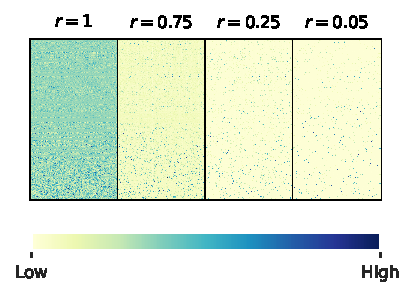
\includegraphics[width = 0.78\columnwidth]{images/subspace_new.pdf}
    \caption{
    \small Visualization of learned final-layer weight matrix for $r \in \{1, 0.75, 0.25, 0.05\}$. For each $r$, we visualize a $342$-dimensional weight vector corresponding to each class in CIFAR-100. }
    \label{fig:subspace}
\end{minipage}%


\end{figure*}
\paragraph{Ablation on subspace dimension.} In this ablation, we aim to empirically verify our theoretical analysis in Section~\ref{sec:theory}, and understand the effect of subspace dimension. 
We start by defining the \textbf{relevance ratio} $r = \frac{s}{m} \in (0,1]$, which captures the sparsity of feature space used in training \name. Recall that $m$ is the original dimension of features and $s$ is the dimension we kept in \name. 

In simple words, $r$ represents the ratio between the dimension of the subspace and the full feature dimension.
Specifically, we train and compare multiple models by varying $r = \{ 0.05, 0.15, 0.25, 0.35, 0.55, 0.75\}$. Figure~\ref{fig:ablations} (left) summarizes the effect of $r$ on OOD detection. We observe that: (1) Irrespective of the relevance ratio used, \name is consistently better than KNN~\cite{sun2022knn} when $r < 1$. This validates the efficacy of learning feature subspaces for OOD detection, without excessive hyperparameter tuning. (2) Setting a mild ratio (\emph{e.g.} $r=0.25$) provides the optimal OOD detection performance, which is consistent with one chosen using our validation strategy (see Appendix C.4). (3) In the extreme case, when $r$ is too small (\emph{e.g.} $r={0.05}$), we observe a deterioration in the OOD detection performance. Overall our empirical observations align well with our theoretical insight provided in Section~\ref{sec:theory}. 

\paragraph{Visualization of the learned weight matrix.}

To further verify our method, we visualize in Figure~\ref{fig:subspace} the 
learned final-layer weight matrix under different relevance ratios ($r = s/m$). For each $r$, we visualize the $342$ dimensional weight vector corresponding to each class in CIFAR-100, \emph{i.e.}, a $342 \times 100$ matrix. When $r=1$ (\emph{i.e.} without any subspace constraint), the model utilizes the full feature space. Further, the visualization confirms that decreasing the relevance ratio effectively reduces feature subspace dimensionality. 

\begin{table}[h]
\centering
\small
\resizebox{0.85\linewidth}{!}{
\begin{tabular}{lccc}
\textbf{Method} & \textbf{FPR95}  & \textbf{AUROC} \\
& $\downarrow $& $\uparrow$ \\
\toprule
Random subspace~\cite{ho1998nearest} & 42.21 & 84.97 \\
Subspace with least relevance & 63.96 & 80.82\\
\name (ours) & \textbf{31.25} & \textbf{90.76} \\
\bottomrule
\end{tabular}}
\caption{\small Ablation on subspace selection methods. Best performing results are marked in \textbf{bold}. Model is DenseNet. All values are averaged over multiple OOD test datasets.}
\label{tab:subspace-selection}
\end{table}


\paragraph{Ablation on subspace selection.} A core component of our algorithm involves selecting the  \emph{most relevant} dimension for a class prediction. In particular, the subspace is chosen based on the dimensions that contributed most to the model's output. In this ablation, we contrast our subspace selection mechanism with random subspace~\cite{ho1998nearest}, a classical alternative. The random subspace relies on a stochastic process that randomly selects $s$ components in the feature vector. Simply put, this approach randomly sets $s$ out of $m$ elements in each $R_c$ vector to be 1 and 0 elsewhere. We report ablation results  in Table~\ref{tab:subspace-selection}. For a fair comparison, we use relevance ratio $r = 0.25$ and the number of neighbors $k = 20$ for all methods.  Empirical results highlight that randomly chosen subsets of dimensions are sub-optimal for the OOD detection task. Lastly, we also contrast with selecting the \emph{least relevant} feature dimensions. We replace Equation~\ref{eq:relevance} with: 
\begin{align}
     f_c(\*x; \theta, R_c(\*x)) & =  \min_{R_c(\*x)\in \{0,1\}^m, \|R_c(\*x)\|_1 = s} \langle \*w_c, h(\*x) \odot R_c(\*x) \rangle,
     \label{eq:least_relevance}
\end{align}
which essentially changes from \textsc{max} to \textsc{min}.  As expected, using the least relevant feature dimension results in significantly worse OOD detection performance.


\paragraph{Ablation on number of nearest neighbors $k$.} 
In Figure~\ref{fig:ablations} (right), we visualize the effect of varying the number of nearest-neighbors ($k$) on OOD detection performance. Here the model is trained with $r=0.25$ on CIFAR-100. Specifically, we vary $k \in \{5,10,20,50,100,200,500,1000\}$. We observe that the  OOD detection performance is relatively stable under a mild $k$. In Appendix D.2, we further visualize the interaction between the two hyper-parameters $r$ and $k$ through OOD detection performance. 

\vspace{0.1cm}
\noindent\textbf{\name improves calibration performance.} {
In addition to superior OOD detection performance, we aim to further  investigate the calibration performance of ID data itself. As a quick recap,  the calibration performance measures the alignment between the model's confidence and its actual predictive accuracy. We hypothesize that learning the feature subspace helps alleviate the problem of over-confident predictions on ID data, thereby improving model calibration. We verify in  Appendix D.3 that training with \name indeed significantly improves the model calibration. }

\vspace{0.1cm}
\noindent\textbf{\name scales to large datasets.} 
In this section, we evaluate \name on a more realistic high-resolution dataset ImageNet ~\cite{deng2009imagenet}. Compared to CIFAR-100, inputs scale up in size in ImageNet-100 (we follow standard data augmentation pipelines and resize the input to 224 by 224). For OOD test datasets, we use the same ones in~\cite{huang2021mos}, including subsets of \texttt{Places365}, \texttt{Textures}, \texttt{iNaturalist} and \texttt{SUN}. 
We train the ResNet-101 model for 100 epochs using a batch size of 256, starting from randomly initialized weights. We use SGD with a momentum of $0.9$, and a weight decay of 1e-4. We set the initial learning rate as $0.1$ and use a cosine-decay schedule. We set $r = 0.35$ and $k = 200$ based on our validation strategy described in Appendix C.4. We contrast two models trained with and without subspace learning. The results in terms of FPR95 and AUROC are shown in Figure~\ref{fig:imagenet}. The results suggest that \name remains effective on all the OOD test sets and consistently outperforms KNN. This further verifies the benefits of explicitly promoting feature subspace to combat curse-of-dimensionality. 

\begin{figure}[t]
    \centering
    \includegraphics[width = \linewidth]{images/imagenet_plot.pdf}
    \caption{\small OOD detection performance comparison on ImageNet dataset (ID). \name consistently outperforms KNN across all OOD test datasets on the same architecture.  }
   
    \label{fig:imagenet}
\end{figure}


